\chapter{Implementación del controlador.}
% ----------------------

\label{C:Implementación del algoritmo de control}
\section{Implementación Física del Algoritmo de Control}
El desarrollo presentado en el capítulo anterior es fundamental para comprender las bases teóricas de las ecuaciones y estrategias que permiten calcular y determinar la acción de control adecuada, con el fin de lograr la mejor respuesta posible en la salida del sistema. Sin embargo, al llevar este algoritmo a una implementación real, es común encontrar variaciones de diseño debido a las condiciones no ideales de los componentes físicos, que difieren de sus contrapartes simuladas en software. En esta sección, se detallan los cambios necesarios para lograr un resultado funcional en la fuente de alimentación tras las pruebas realizadas con el primer prototipo, lo que condujo al diseño final.\par

\subsection{Condiciones de Funcionamiento}
Uno de los aspectos clave en el diseño de la fuente es la necesidad de garantizar que la magnitud de salida se mantenga estable a lo largo del tiempo, independientemente de las condiciones de carga. En este contexto, se identifican dos escenarios típicos: cuando hay una carga conectada a la salida y cuando no la hay. \par
Existe una diferencia significativa entre estos dos escenarios, ya que afectan el comportamiento del capacitor de salida, lo que a su vez determina cómo se disipa la energía. En presencia de una carga, el capacitor se descarga más rápidamente, dado que existe un consumo constante de energía. Por el contrario, en ausencia de carga, la descarga del capacitor ocurre a un ritmo más lento, ya que las resistencias \textit{R\textsubscript{SHUNT}} no son el medio ideal para drenar la energía. \par

\subsection{Rangos de Funcionamiento}
Otro aspecto a considerar es la necesidad de asegurar una respuesta transitoria relativamente rápida para cualquier valor de tensión seteado en la salida. La eficiencia del algoritmo de control no es igual cuando se ajusta una referencia de 5V en comparación con una de 30V. Por lo tanto, las constantes que determinan la intensidad de la acción de control deben ser ajustadas de manera diferente en cada caso para optimizar el rendimiento.\par

\subsection{Determinación de Escenarios}
El algoritmo de control implementado en la fuente de alimentación utiliza un criterio específico para determinar si hay una carga conectada o si el circuito se encuentra en una condición de vacío. Este criterio se basa principalmente en la evaluación de los valores de corriente medidos en la salida de la fuente. Si la corriente tiende a cero, el algoritmo concluye que el circuito está abierto, interpretando esta situación como una condición de vacío. En contraste, si se detecta una corriente significativa, se determina que existe una carga conectada.\par
Otro parámetro crucial en la determinación de los escenarios es el comportamiento de la tensión una vez que se ha estabilizado. Un aumento rápido en el valor de la tensión sugiere que una carga ha sido desconectada de manera repentina, mientras que una disminución en la tensión de salida indica que se ha producido una perturbación o que se ha añadido otra carga en paralelo. Estos cambios en la tensión permiten al algoritmo identificar la transición entre diferentes estados operativos.\par
Con base en estos criterios, el sistema evalúa la situación actual de la fuente y, en consecuencia, selecciona las constantes del controlador que se deben aplicar en el algoritmo para optimizar la respuesta.\par

\section{Estrategia Empleada en el Algoritmo}
La combinación de las condiciones de carga y los amplios rangos de funcionamiento llevó al desarrollo de una matriz de control de 6x12. Esta matriz define los valores de las constantes del controlador en función del valor de referencia y de la presencia o ausencia de carga en la salida. Para cada condición, se emplean tres constantes que gobiernan el lazo de corriente y tres constantes adicionales para el lazo de tensión, con una separación de 5V entre las constantes abarcando un rango de 0 a 30V. Esta estrategia permite obtener una respuesta transitoria más ajustada a los diferentes valores deseados.\par
Estas medidas fueron implementadas debido a la complejidad inherente al diseño de la fuente y con el objetivo de realizar múltiples optimizaciones en el control eficiente del sistema. La implementación de esta estrategia asegura que la fuente pueda adaptarse dinámicamente a las distintas condiciones operativas, garantizando un rendimiento superior en una variedad de escenarios.\par

\begin{figure}[H]
    \centering
    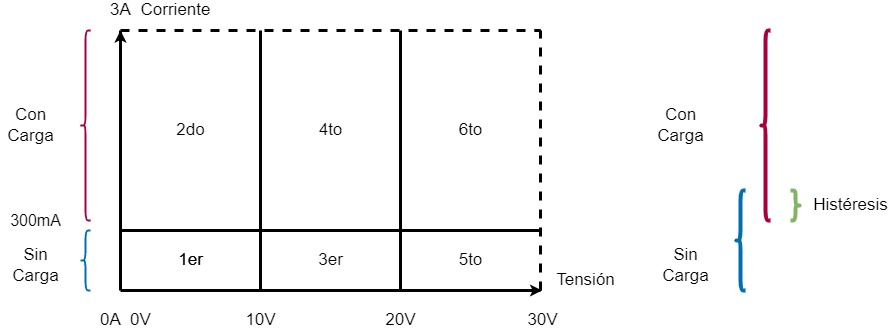
\includegraphics[scale=0.5]{./imagenes/matriz.jpg}
    \caption{Matriz de constantes de controlador.}
    \label{F:matriz_control}
\end{figure}

\subsection{Soft Reset}
Para evitar la malinterpretación de las variables durante la transición entre estados de carga y sin carga, se implementó un \textit{soft reset} en el algoritmo de control. Dado que las variables del algoritmo afectan a ambos estados de manera similar, este \textit{soft reset} previene efectos indeseados en las magnitudes de salida. Al ejecutar un \textit{soft reset} durante estas transiciones, se provoca una breve caída en la tensión de salida, lo que permite reiniciar el sistema desde un punto de referencia de 0V y, de esta manera, lograr una curva de respuesta adecuada para las diferentes condiciones de carga que puedan presentarse.

\subsection{Protección Ante Sobretensiones y Falso Contacto}
En sistemas electrónicos, es común que las cargas puedan tolerar un valor de alimentación inferior al diseñado durante unos pocos milisegundos, hasta que la tensión alcanza su valor nominal. Sin embargo, esta tolerancia no se extiende a las sobretensiones, ya que incluso una sobretensión de corta duración puede ser suficiente para dañar los componentes electrónicos de una carga. Por esta razón, se ha implementado en la fuente de alimentación una protección contra sobretensiones que desconecta inmediatamente el relé de salida al detectar un valor de tensión superior al permitido.\par
Una vez que la sobretensión ha sido eliminada y la tensión de salida se ha estabilizado dentro de los límites predefinidos durante un tiempo determinado, el relé de salida se vuelve a habilitar, permitiendo nuevamente el acoplamiento de la carga. Esta función es particularmente útil en situaciones donde se produce un falso contacto, que puede generar picos de tensión y perturbaciones en la salida de la fuente. De este modo, se ofrece una protección adicional para la carga, garantizando su integridad ante escenarios potencialmente dañinos.\par
Este mecanismo de protección no solo previene daños permanentes en los dispositivos conectados, sino que también asegura una mayor durabilidad y fiabilidad del sistema en su conjunto, al minimizar los riesgos asociados con fluctuaciones de tensión imprevistas. \par
